\usetikzlibrary{patterns}
\begin{figure}[ht]
    \centering
   


% Pattern Info
 
\tikzset{
pattern size/.store in=\mcSize, 
pattern size = 5pt,
pattern thickness/.store in=\mcThickness, 
pattern thickness = 0.3pt,
pattern radius/.store in=\mcRadius, 
pattern radius = 1pt}
\makeatletter
\pgfutil@ifundefined{pgf@pattern@name@_v5u0tibg}{
\pgfdeclarepatternformonly[\mcThickness,\mcSize]{_v5u0tibg}
{\pgfqpoint{0pt}{0pt}}
{\pgfpoint{\mcSize+\mcThickness}{\mcSize+\mcThickness}}
{\pgfpoint{\mcSize}{\mcSize}}
{
\pgfsetcolor{\tikz@pattern@color}
\pgfsetlinewidth{\mcThickness}
\pgfpathmoveto{\pgfqpoint{0pt}{0pt}}
\pgfpathlineto{\pgfpoint{\mcSize+\mcThickness}{\mcSize+\mcThickness}}
\pgfusepath{stroke}
}}
\makeatother
\tikzset{every picture/.style={line width=0.75pt}} %set default line width to 0.75pt        

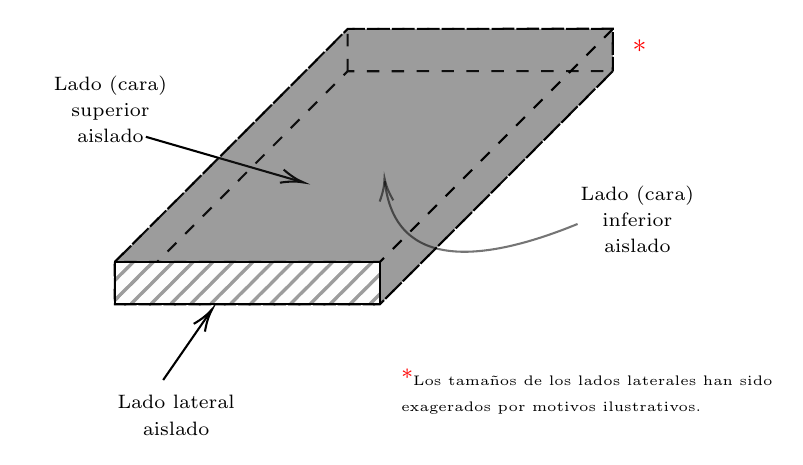
\begin{tikzpicture}[x=0.75pt,y=0.75pt,yscale=-1,xscale=1]
%uncomment if require: \path (0,300); %set diagram left start at 0, and has height of 300

%Shape: Cube [id:dp5983494268286695] 
\draw  [fill={rgb, 255:red, 0; green, 0; blue, 0 }  ,fill opacity=0.39 ][dash pattern={on 4.5pt off 4.5pt}] (420.4,60.04) -- (308.23,172.37) -- (180.47,172.46) -- (180.46,152.05) -- (292.63,39.72) -- (420.38,39.63) -- cycle ; \draw  [dash pattern={on 4.5pt off 4.5pt}] (180.47,172.46) -- (292.65,60.13) -- (420.4,60.04) ; \draw  [dash pattern={on 4.5pt off 4.5pt}] (292.65,60.13) -- (292.63,39.72) ;
%Straight Lines [id:da8348539716971336] 
\draw    (195.43,91.71) -- (269.51,113.16) ;
\draw [shift={(271.43,113.71)}, rotate = 196.14] [color={rgb, 255:red, 0; green, 0; blue, 0 }  ][line width=0.75]    (10.93,-3.29) .. controls (6.95,-1.4) and (3.31,-0.3) .. (0,0) .. controls (3.31,0.3) and (6.95,1.4) .. (10.93,3.29)   ;
%Straight Lines [id:da814133806997101] 
\draw    (203.78,208.88) -- (226.29,176.36) ;
\draw [shift={(227.43,174.71)}, rotate = 484.69] [color={rgb, 255:red, 0; green, 0; blue, 0 }  ][line width=0.75]    (10.93,-3.29) .. controls (6.95,-1.4) and (3.31,-0.3) .. (0,0) .. controls (3.31,0.3) and (6.95,1.4) .. (10.93,3.29)   ;
%Shape: Cube [id:dp7512885899814816] 
\draw  [fill={rgb, 255:red, 155; green, 155; blue, 155 }  ,fill opacity=0.1 ][dash pattern={on 4.5pt off 4.5pt}] (180.47,151.96) -- (292.72,39.71) -- (420.47,39.71) -- (420.47,60.12) -- (308.23,172.37) -- (180.47,172.37) -- cycle ; \draw  [dash pattern={on 4.5pt off 4.5pt}] (420.47,39.71) -- (308.23,151.96) -- (180.47,151.96) ; \draw  [dash pattern={on 4.5pt off 4.5pt}] (308.23,151.96) -- (308.23,172.37) ;
%Curve Lines [id:da2881177340231348] 
\draw [color={rgb, 255:red, 0; green, 0; blue, 0 }  ,draw opacity=0.54 ]   (403.43,133.71) .. controls (359.87,151.53) and (315.33,157.59) .. (310.56,113.08) ;
\draw [shift={(310.43,111.71)}, rotate = 445.03] [color={rgb, 255:red, 0; green, 0; blue, 0 }  ,draw opacity=0.54 ][line width=0.75]    (10.93,-3.29) .. controls (6.95,-1.4) and (3.31,-0.3) .. (0,0) .. controls (3.31,0.3) and (6.95,1.4) .. (10.93,3.29)   ;
%Shape: Rectangle [id:dp15714361951792954] 
\draw  [color={rgb, 255:red, 0; green, 0; blue, 0 }  ,draw opacity=1 ][pattern=_v5u0tibg,pattern size=7.199999999999999pt,pattern thickness=3.75pt,pattern radius=0pt, pattern color={rgb, 255:red, 253; green, 253; blue, 253}] (180.47,151.96) -- (308.23,151.96) -- (308.23,172.37) -- (180.47,172.37) -- cycle ;

% Text Node
\draw (139,60.79) node [anchor=north west][inner sep=0.75pt]  [font=\footnotesize] [align=left] {\begin{minipage}[lt]{56.822500000000005pt}\setlength\topsep{0pt}
\begin{center}
{\scriptsize Lado (cara) superior }\\{\scriptsize aislado}
\end{center}

\end{minipage}};
% Text Node
\draw (395,113.79) node [anchor=north west][inner sep=0.75pt]  [font=\footnotesize] [align=left] {\begin{minipage}[lt]{53.58643005371094pt}\setlength\topsep{0pt}
\begin{center}
{\scriptsize Lado (cara) inferior }\\{\scriptsize aislado}
\end{center}

\end{minipage}};
% Text Node
\draw (173,214.79) node [anchor=north west][inner sep=0.75pt]  [font=\footnotesize] [align=left] {\begin{minipage}[lt]{53.27071502685547pt}\setlength\topsep{0pt}
\begin{center}
{\scriptsize Lado lateral aislado}
\end{center}

\end{minipage}};
% Text Node
\draw (317,201.79) node [anchor=north west][inner sep=0.75pt]  [font=\footnotesize] [align=left] {\textcolor[rgb]{1,0,0}{*}{\tiny Los tamaños de los lados laterales han sido }\\{\tiny exagerados por motivos ilustrativos.} };
% Text Node
\draw (428.43,43.5) node [anchor=north west][inner sep=0.75pt]   [align=left] {\textcolor[rgb]{1,0,0}{*}};


\end{tikzpicture}
   \caption{Placa rectangular metálica}
\end{figure}